%
%	Begrifflichkeiten
%

\pagebreak
\section{Targeting}

\onehalfspacing

\subsection{Targeted Advertising}

\subsubsection{Rationale}

Why do we need targeted advertising?

"Microtargeting is a marketing strategy that uses people’s data — about what they like, who they’re connected to, what their demographics are, what they’ve purchased, and more — to segment them into small groups for content targeting. It’s the reason that if you typically shop at Whole Foods, you may be served an advertisement for organic sunscreen during the Summer. And while it can help deliver content that is interesting and helpful to you, it also has a dark side — especially if it delivers information that’s inaccurate or biased and meant to sway your vote."\footnote{\textit{Ghosh, D. (2018)}: What is microtargeting? \cite{mozillaBlog}}

\subsubsection{Tracking}

Tracking is under attack from multiple angles\footnote{See \textit{Brinkmann, M. (2021)}: How Firefox new SmartBlock feature works \cite{mozillaBlog}}

Even Google, who invented various tracking methods, will no longer support it in Chrome.

\subsubsection{Cookies}

We will focus on Cookies and web browser as the main tracking mechanisms.

A cookie is a small piece of information that a server sends to the user's web browser for storage, and which it can request back at a later point in time.

Cookies can be used for session management, personalizing and tracking.\footnote{See \textit{Mozilla (2021)}: Using HTTP cookies \cite{usingCookies}}

There's also tracking in E-Mail\footnote{See \textit{Doffmann, Z. (2021)}: Why You Suddenly Need To Delete Gmail On Your iPhone \cite{deleteGmail}}, which we will ignore for this paper.

\subsection{Data Types}

\subsubsection{First-Party Data}

First party data is data that we collect from our own sources.\footnote{See \textit{OnAudience (2019)}: What is first party data? \cite{firstParty}}

\subsubsection{Second-Party Data}

Second party data is another companies first party data.\footnote{See \textit{OnAudience (2019)}: What is first party data? \cite{firstParty}}

\subsubsection{Third-Party Data}

Third party data is additional data that you buy from specialized sources on the web to enrich your own data.\footnote{See \textit{OnAudience (2019)}: What is first party data? \cite{firstParty}}

\subsection{Tool-stack - Analytics}

\subsubsection{Google Analytics}

\href{https://analytics.google.com/}{Google Analytics} gives you all the tools to analyze your web business data and gain insights into your campaign performances.

\subsubsection{Open Source Analytics}

In addition to Google Analytics, there are a couple of open source alternatives, one of which is Plausible.\footnote{See \textit{Frank, C. (2020)}: Usefulness of open-source tools for web analytics in EMarketing \cite{previousPaper}} 

\begin{figure}[H]
\centering
\caption {Plausible}
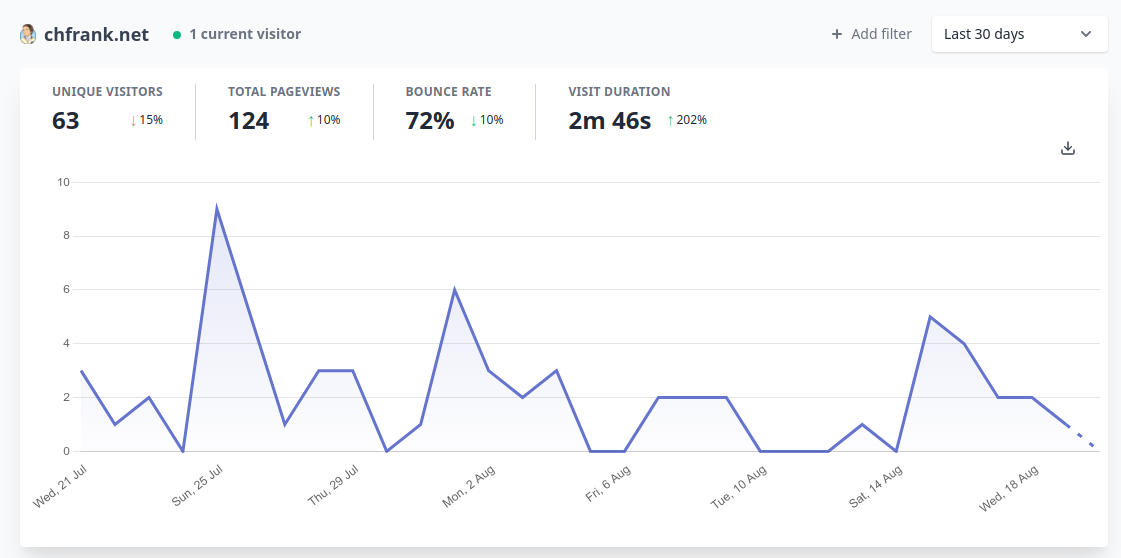
\includegraphics[width=\linewidth]{images/plausible.png}
\label{fig:plausible}
\end{figure}

Looking at the data provided, we can gather deep insights into the visitors of our page and predict the performance of our campaigns.\footnote{See \textit{Frank, C. (2021)}: Web Traffic Analysis - Predicting Blog Post Performance \cite{previousBigdata}}

We can also analyze key performance indicators for our campaigns, such as Click-Through or Conversion rates.\footnote{See \textit{Romes, Y. (2020)}: 10 Inbound KPIs, die jetzt auch Personaler kennen sollten \cite{inboundKPI}}

\subsubsection{Yandex Metrica}

\href{https://metrica.yandex.com/}{Yandex Metrica} is another commercial option for web page analytics, located in Russia.

\subsection{Tool-stack - Advertising}

\subsubsection{Google Ads}

\href{https://ads.google.com/home/}{Google Ads} is a platform to place ads on Google's pages and affiliates.

Placement and Algorithm is a science unto itself; recently Google has come under scrutint from the regulators and in one case, agreed to the ruling and the fine.\footnote{See \textit{Burgess, M. (2021)}: France Cracked Down on Google’s Ad Tech \cite{googleAds}}

\subsubsection{Amazon Advertising}

\href{https://advertising.amazon.com//}{Amazon Advertising} is a platform to place ads for your products on Amazon's pages.

\subsubsection{Facebook Advertising}

\href{https://www.facebook.com/business/ads}{Facebook Ads} is a platform to place ads on Facebook's pages and affiliates.

\subsection{Moving past cookies}

\subsubsection{Browser-based}

To continue with targeted advertising, even after the demise of the tracking cookie, a new concept of Privacy Preserving Advertising has emerged.\footnote{See \textit{Rescorla, E. (2021)}: The future of ads and privacy \cite{futureAds}}

The primary contender in this space is \href{https://wicg.github.io/floc/}{Google FLoC}, which is under fire from a privacy point of view.\footnote{See \textit{Rescorla, E. (2021)}: Privacy analysis of FLoC \cite{privacyFloc}} Among others, EFF has published a detailed analysis of FLoC's shortcomings in regards to privacy and why they believe that FLoc would be a terrible idea.\footnote{See \textit{Cyphers, B. (2021)}: Google’s FLoC Is a Terrible Idea \cite{terribleIdea}}

\subsubsection{Data-based}

A second approach is based around data clean rooms, to enable the combination of first party data with second party data, without running afoul of data protection regulations.\footnote{See \textit{Younger, M. (2019)}: The Three Hidden Technology Trends Behind Data Clean Rooms \cite{cleanRoom}}

\subsubsection{Identity-based}

Similar to FLoC are several other approaches to implement some kind of advertising ID, that would attempt to not violate the user's privacy rights but still allow for targeted advertising. The most promising approach was Apple's ID for Advertising, which seems to be not going anywhere for the time being.\footnote{See \textit{Ray, O. (2020)}: What is IDFA and Why Apple Killed it \cite{cleanRoom}}

\subsubsection{Content-based targeting}

In 2020, the public radio in The Netherlands went from targeted advertising to contextual advertising and saw their ad revenues grow.\footnote{See \textit{Edelman, G. (2020)}: Can Killing Cookies Save Journalism? \cite{killingCookies}} 

The system at \href{https://over.npo.nl/}{NPO} is a bidding system similar to Google Ads, however, ads are not placed based on a user profile but the current context, i.e. a web page shown or a TV show watched.

\subsection{Legal Framework}

There's a number of legal frameworks that govern tracking and advertising, here's a list of the most common ones with links to the legal texts:

\begin{itemize}
 \item \href{https://gdpr-info.eu/}{GDPR} (General Data Protection Regulation)
 \item \href{https://www.datenschutz-grundverordnung.eu/}{DSGVO} (Datenschutzgrundverordnung)
 \item \href{https://dsgvo-gesetz.de/ttdsg/}{TTDSG} (Telekommunikations-Telemedien-Datenschutz-Gesetz (Entwurf ))
 \item \href{https://oag.ca.gov/privacy/ccpa}{CCPA} (California Consumer Privacy Act)
 \item \href{https://www.lgpdbrasil.com.br/}{LGPD} (Lei Geral de Proteção de Dados Pessoais)
 \item \href{https://popia.co.za/}{POPIA} (Protection of Personal Information Act)
 \item \href{https://ec.europa.eu/info/strategy/priorities-2019-2024/europe-fit-digital-age/digital-services-act-ensuring-safe-and-accountable-online-environment_en}{DSA} (Digital Services Act)
 \item \href{https://ec.europa.eu/info/strategy/priorities-2019-2024/europe-fit-digital-age/digital-markets-act-ensuring-fair-and-open-digital-markets_en}{DMA} (Digital Markets Act)
\end{itemize}

In this paper, we will assume that the reader is familiar with the content of the various regulations and solely focus on their impact and interpretation.
